\newpage
\chapter{Umsetzung}

\section{Implementierung}

\subsection{Server}

\subsubsection{Handling Drohnen Kommunikation}

In der Architektur ist beschrieben, dass die Drohnen über AMQP mit dem Messaging-Broker kommunizieren. Um die Möglichkeit zu haben mit einzelnen Drohnen zu kommunizieren, müssen auf dem Server zur Laufzeit alle Verbindungen zu allen Drohnen bekannt sein. Ausserdem muss en möglich sein, eingehende Nachrichten an einem zentralen Punkt abzuarbeiten. Auf Grund der bestehenden MVC-Struktur der Play-Applikation haben wir uns entschieden, auch die Nachrichten aus dem Messaging-System in Controllern zu behandeln, wie es normalerweise nur mit HTTP-Requests geschieht.

Die Abbildung \ref{fig:drone-communication-diagram} zeigt ein Objekt-Diagramm von Instanzen, die die Kommunikation mit den Drohnen erlauben, sobald die Applikation gestartet hat.

\begin{figure}[H]
	\centering
	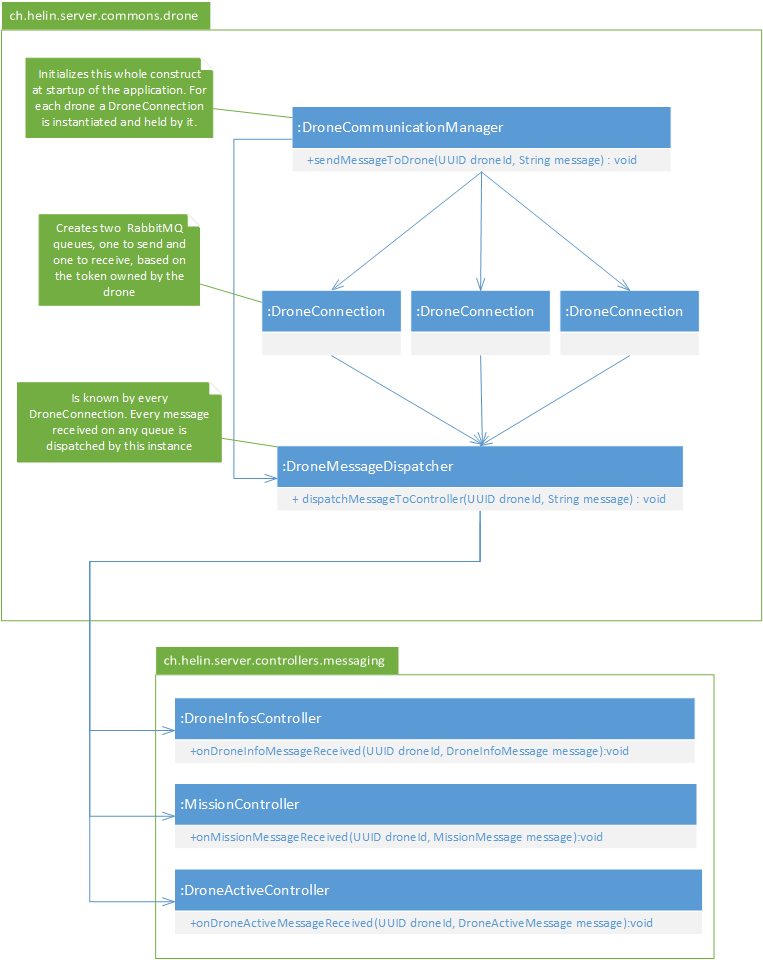
\includegraphics[width=0.8\paperwidth] {images/drone-communication-diagram.png}
	\caption{Objekt-Diagramm der Kommunkationsstruktur}
	\label{fig:drone-communication-diagram}
\end{figure}

\subsubsection{Verwendete Bibliotheken}
\begin{tabularx}{\textwidth}{|X|X|c|X|}
	\hline
	\textbf{Name} & \textbf{Verwendungszweck} & \textbf{Version} & \textbf{Lizenz} \\
	\hline \hline
	Hibernate ORM Mapper & Objekt-Relationales mapping zwischen Datenbank und Models  & 5.1.0 & Apache 2.0\\
	\hline 
	RabbitMQ Client & Client Komponente zur Kommunikation mit dem Rabbit MQ Server & 3.6.0 &  Mozilla Public License 1.1, GPL 2, Apache 2.0 \\
	\hline 
	jGraphT & Graph Bibliothek für Java, um effizient Operationen auf dem Graph auszuführen & 0.9.2 &  LGPL, EPL \\
	\hline 
	\hline
	\textbf{Name} & \textbf{Verwendungszweck} & \textbf{Version} & \textbf{Lizenz} \\
	\hline \hline
	Google GSON & Java Serialisierungs / Deserialisierungs Bibliothek & 2.6.2 & Apache 2.0\\
	\hline 
\end{tabularx}

\subsection{Onboard-App}


\subsection{Kommunikation}
Um die nichtfunktionalen Anforderungen im Bereich der Kommunikation zu erfüllen, wurde AMQP als Protokoll ausgewählt. Mit Messaging soll gewährleistet werden, dass die Verbindungswiederherstellung funktioniert. Die funktionale Anforderung des Missionsabbruchs wird somit soweit gedeckt, dass versucht wird die Verbindung aufrechtzuerhalten, sofern das Netz es erlaubt. Bei kurzen Netzunterbrüchen kann somit über das AMQP Protokoll eine Verbindung zur Drohne gewährleistet werden.

\begin{itemize}
	\item{\textbf{Verbindungsabbruch:} \\
		Gemäss den nicht funktionalen Anforderungen darf der Verbindungsabbruch keinen Einfluss auf die Mission haben. Um gemäss den funktionalen Anforderungen einen Missionsabbruch zu gewährleisten, wird versucht Unterbrüche so kurz wie möglich zu halten und einen automatischen Verbiundungsaufbau zu ermöglichen. Aus diesem Faktoren wird die gesamte Mission vor dem Start übertragen, damit sie ausgeführt werden kann. Einzelne Wegpunke sind somit nicht auf eine stabile Internetverbindung angewiesen, da die Route bereits von Anfang bekannt ist. Der Missionsabbruch ist ebenfalls gewährleistet - sofern die GSM Verbindung besteht. 
		\\
		Verbindungsabbrüche auf dem Mobiltelefon haben zweierlei Konsequenzen:	
		\begin{itemize}
			\item{\textbf{Mobiltelefon kann die Messages vom Server nicht empfangen:} \\
				Dieses Szenario wird durch das RabbitMQ abgefangen. Der Messaging Broker cached die Nachrichten solange bis der Consumer (Mobiltelefon) wieder verfügbar ist. Es besteht somit kein zusätzlicher Handlungsbedarf auf dem Onboard-App.
			}
			\item{\textbf{Messages vom Mobiltelefon zum Server können nicht gesendet werden:} \\
				In diesem Fall kann der Übertragungsfehler nicht durch RabbitMQ abgefangen werden. Der Broker hat vom Producer (Mobiletelefon) noch keine Nachricht bekommen. Aus diesem Grund wird producerseitig eine Exception geworfen, die darauf hinweist, dass die Verbindung unterbrochen ist. In diesem Fall wird die Nachricht in einem Queue zwischengespeichert. Sämtliche Folgenachrichten, die während des Verbindungsunterbruchs nicht übertragen werden können, werden ebenfalls in dieser Queue gespeichert. Sobald die Verbindung wieder besteht, werden die Nachrichten aus der Queue gesendet.
			}
		\end{itemize}
		Mit diesen Massnahmen ist ein guter Kompromiss aus Zuverlässigkeit und Aufwand entstanden. Alle missionskritischen Nachrichten können übertragen werden. Telemetriedaten sind von einem Verbindungsausfall ebenfalls nicht betroffen.
	}
	\item{\textbf{Verbindungswiederherstellung:}
		Aus den nicht funktionalen Anforderungen ist zu entnehmen, dass bei einem Verbindungsunterbruch ein Reconnect statt findet. Dieser Reconnect soll, sobald die Verbindung im GSM Netz wieder besteht nicht länger als 30s dauern. \\
		Bei der Konfiguration von AMQP bestanden mehrere Möglichkeiten. Einersetis war der bekannte Backoff Algorithmus eine Option. Dieser Algorithmus arbeitet nach einem incrementellen Prinzip. Je länger der Unterbruch dauert, desto länger dauert es bis er die Verbindung wieder versucht aufzubauen. Auf der anderen Seite stand ein einfacher Interval-Algorithmus. Dieser versucht alle drei Sekunden die Verbindung wiederherzustellen, bis zum erfolgreichen Verbindungsaufbau. Mit diesen Erkenntnissen haben wir folgende Messung gemacht:
		\begin{center}
			\begin{tabular}{|r|r|}
				\hline
				\textbf{Backoff} & \textbf{Interval 3s} \\
				\hline
				17 & 7 \\
				7 & 7 \\
				9 & 7 \\
				11 & 7 \\
				10 & 7 \\
				\hline
				% TODO: Kommentar noch: Anzahl Sekunden bis zum Verbindungsaufbau
			\end{tabular}
		\end{center}
		Aus diesen Erkenntnissen standen beide Möglichkeiten offen, denn beide erfüllen die Anforderungen und haben somit auch keine Auswirkungen auf die Qualität. Am Ende wurde bewusst auf den BackOff Algorithmus gesetzt. Der Backoff Algorithmus benötigt zwar deutlich länger für einen Reconnect als das fixe Zeitinterval. Die hetrogene Verteilung der Wiederverbindungszeiten spricht aber für den Backoff Algorithmus. Sollte es zu Probleme auf der Serverseite kommen, so werden nicht alle Geräte gleichzeitig einen Reconnect probieren - der Reconnect passiert somit gestaffelt. Dies bringt zusätzlich Stabilität ins System.}
	\item{\textbf{Android Process Lifecycle:} \\
		Da die OnboardApp auf einem Android Betriebssystem läuft, mussten gewisse Voraussetzungen geprüft werden. Im Grund kann davon ausgegangen werden, dass die Applikation immer im Vordergrund steht. Es ist doch sehr unwahrscheinlich, dass die Appliaktion in den Hintergrund rückt, weil eine andere Applikation verwendet wird. \\
		Laut Android Dokumentation ist das Verhalten einer Applikation im Hintergrund nicht deterministisch \cite{androidGuide}. Sollte eine Applikation im Hintergrund gewisse Garantien haben, so muss von einem Service und der spezifischen Implementierung eines Services gesprochen werden. Im Fall der OnboardApp und den getroffenen Annahmen, wurde davon abgesehen, da die Applikation während des Fluges nicht gewechselt wird.
	}
	\newpage
\end{itemize}

\subsection{Sicherheit}
Wie sicher ist die Kommunikation mit dem Server? Kann allenfalls eine Drohne gekapert und falsche Koordinate zugeschickt werden?
\\
Die Verbindung zum RabbitMQ läuft über TLS (Transport Layer Security ). 
Die Kommunikation mit dem Server läuft über zwei Queues:
\begin{itemize}
	 \item \{token\}-Drone-To-Server
	 \item  \{token\}-Server-To-Drone
\end{itemize}

Beim Token handelt es sich um einen auf dem Smartphone gespeicherten UUID, welcher vom Server beim erstmaligen Anmelden zugewiesen wird.
Über diesen Kanal werden JSON Messages ausgetauscht. Ein Angreifer müsste den Token herausfinden. Mit einer Brutforce Methode ist mit $2^122$ Möglichkeiten ein Treffer auszuschliessen. 
Da bei der Anmeldung der Drohne die Verbindung über HTTPS ist, kann auch das auslesen des Tokens ausgeschlossen werden.
Somit ist für uns die Kommunikation mit der Drohne ausreichend gesichert.


\subsubsection{Verwendete Bibliotheken}
\begin{tabularx}{\textwidth}{|X|X|c|X|}
	\hline
	\textbf{Name} & \textbf{Verwendungszweck} & \textbf{Version} & \textbf{Lizenz} \\
	\hline \hline
	DroneKit-Android Client & Android API für MAV-Link Protokoll zum ansteuern der Drohne & 1.5.1 & Apache 2.0\\
	\hline 
	AMQP Messaging Library & Messaging für Android & 3.6.0 &  Mozilla Public License 1.1, GPL 2,  Apache 2.0 \\
	\hline 
	Lyra  & High availability Messaging & 0.4.3 &  Apache 2.0 \\
	\hline 
\end{tabularx}
\subsection{Customer App}
Gemäss Aufgabenstellung sollte ein Prototyp für eine App, mit welchem Bestellungen am System abgegeben können, entwickelt werden.
Diese App wurde als letzte Komponente entwickelt, da sie erst getestet werden konnte als die Server- und Onboard-App-Komponenten fertiggestellt waren.

Um manuelle Tests der Bestell-API möglich zu machen, wurde in der Administrations-Seite eine "'Fake Order"' Funktionen eingeführt. 
Diese imitiert eine Bestellung des Kunden und schickt eine Anfrage mit vordefinierten Koordinaten und Produkten an das System.

\begin{figure}[H]
	\centering
	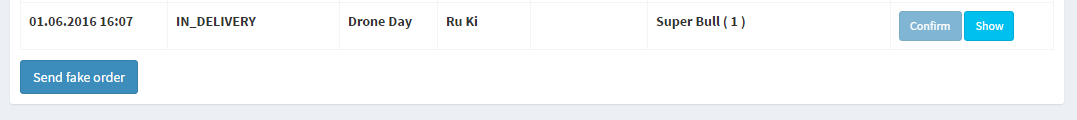
\includegraphics[width=1\textwidth] {images/customer-app-fake-order.png}
	\caption{Send Fake Order within Administrator Page}
\end{figure}

Anders als die Onboard-App, welche native mit Java entwickelt wurde und nur auf Android läuft, entschieden wir uns beim Bestell-App für eine Cross-Plattform Lösung, welche Android und iOS unterstützt. 

Auch wenn gemäss der Aufgabenstellung keine iOS App gefordert war, stelle sich doch die Frage ob man die iPhone-Kunden ausschliessen soll und spätere Entwickler zwingt, einen grossen Teil des Codes in einer nativen iOS App duplizieren zu müssen. Mit einem Marktanteil von 42.2\% (Zahlen 2015) \cite{ios-user} von iOS Benutzern in der Schweiz, ist anzunehmen, dass zu einem späteren Zeitpunkt eine iPhone App implementiert werden muss.

Deshalb wurde auf Xamarin Forms gesetzt, welches ermöglicht, die ganzen Service-Klassen und einen Teil der Benutzeroberfläche für die verschiedenen Plattformen nur einmal zu implementieren.

Die App wurde in einer minimalen Ausbaustufe erstellt, erfüllt aber bereits alle nötigen Funktionalen Anforderungen. In Abbildung \ref{fig:customer-app-flow} wird gezeigt, wie ein Benutzer durch die App navigieren kann. 

Besonders wichtig ist die Anzeige des berechneten Abwurfpunktes vor der Bezahlung der Ware, sowie die Anzeige der Drohnenposition in Echtzeit während des Anflugs der Drohne.  

\begin{landscape}
	\begin{figure}[h]
		\centering
		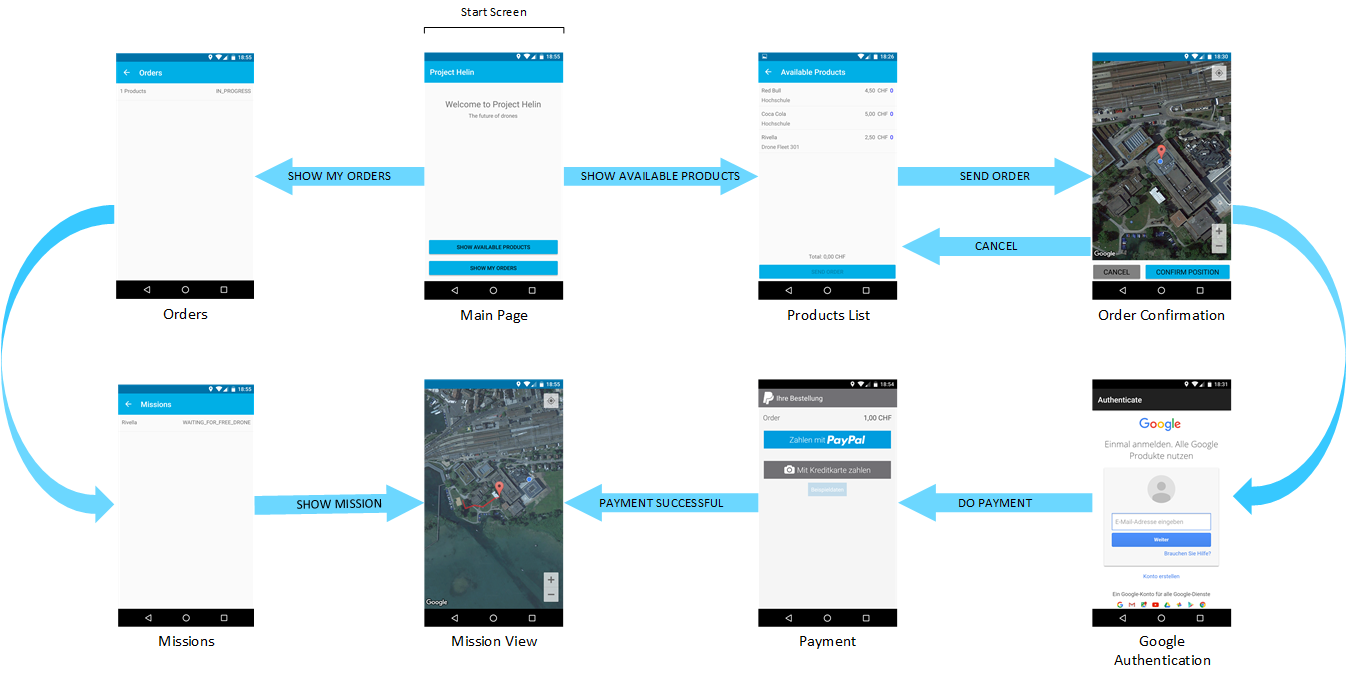
\includegraphics[width=0.8\paperheight] {images/customer-app-pages.png}
		\caption{Übersicht der Customer App mit allen Verknüpfungen zwischen den Screens}
		\label{fig:customer-app-flow}
	\end{figure}
\end{landscape}

\subsubsection{Verwendete Bibliotheken}
\begin{tabularx}{\textwidth}{|X|X|c|X|}
	\hline
	\textbf{Name} & \textbf{Verwendungszweck} & \textbf{Version} & \textbf{Lizenz} \\
	\hline \hline
	Paypal Forms & Paypal integration für Xamarin.Forms & 2.0.4 & MIT \\
	\hline 
	Xamarin Forms & Plattform übergreifende Komponente für Xamarin & 2.2.0.45 & \url{https://www.xamarin.com/license} \\
	\hline 
	Websocket.PCL & Plattformübergreifende Websocket Anbindung & 1.1.9 & MIT \\
	\hline 
	Newton.Json & Json zu Object mapper & 8.0.3 & MIT \\
	\hline 
\end{tabularx}



\section{Projektgrösse}

Folgende Statistiken wurden am Ende der Arbeit erstellt um einen Eindruck der Grösse des Projekts zu erhalten.\\

\begin{figure}[H]
	\centering
	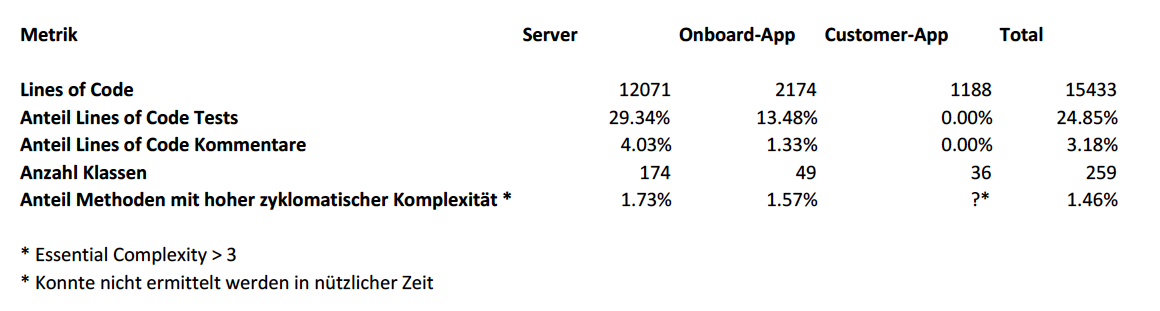
\includegraphics[width=1.0\textwidth] {images/code-metrics.png}
	\caption{Code Metriken nach Abschluss der Arbeit}
	\label{fig:code-metrics}
\end{figure}

In Abbildung \ref{fig:code-metrics} sind vor allem der geringe Anteil von Methoden mit hoher Essentieller Komplexität hervorzuheben. Alle Methoden mit hoher Komplexität wurden vom Team geprüft, konnten aber nicht mehr verbessert werden. Hauptsächlich sind dies 'equals' Methoden von grösseren DTOs oder es handelt sich um MessageConverter, die einfach alle verschiedenen Messagetypen verschieden behandeln müssen. Das folgende Beispiel zeigt die Methode mit der höchsten Zyklomatischen Komplexität der Server-Applikation (Essentielle Komplexität = 10, Cyclomatische Komplexität = 10). \\


\begin{lstlisting}
private Message parseMessageWithoutCare(String messageAsJson) {
	...
	switch (payloadType) {
		case ConfirmCargoLoaded:
			return gson.fromJson(messageAsJson, ConfirmCargoLoaded.class);
		case NotifyCargoDrop:
			return gson.fromJson(messageAsJson, NotifyCargoDrop.class);
		case DroneInfo:
			return gson.fromJson(messageAsJson, DroneInfoMessage.class);
		case DroneDto:
			return gson.fromJson(messageAsJson, DroneDtoMessage.class);
		case AssignMission:
			return gson.fromJson(messageAsJson, AssignMissionMessage.class);
		case FinalAssignMission:
			return gson.fromJson(messageAsJson, FinalAssignMissionMessage.class);
		case ConfirmMission:
			return gson.fromJson(messageAsJson, ConfirmMissionMessage.class);
		case FinishedMission:
			return gson.fromJson(messageAsJson, FinishedMissionMessage.class);
		case DroneActiveState:
			return gson.fromJson(messageAsJson, DroneActiveStateMessage.class);
	}
}

\end{lstlisting}

Da diese Methode gut strukturiert ist und auch gut verstanden werden kann, gibt es keinen Grund diese auf Grund der Metrik anzupassen.

\section{Qualitätssicherung}

\subsection{Prozesse}

Zur Qualitätssicherung wurde im Projektmanagement-Tool neben Todo, In Progress und Done ein neuer Quality-Assurance-Status für die Issues eingeführt. Alle Issues in diesem Status mussten von einem anderen Teammitglied überprüft werden, bevor sie auf Done geschoben werden konnten. \\

Die Überprüfung eines Issues beinhaltet folgende Aufgaben:

\begin{itemize}
	\item{Akzeptanzkriterien aus der User-Story manuell prüfen}
	\item{Code-Review durchführen (Intensität je nach Grösse und Komplexität des geschriebenen Codes)}
	\item{Code auf Vertösse gegen Style-Guide prüfen}
\end{itemize}

Damit konnten viele Fehler früh entdeckt werden und die Code-Qualität konnte über die ganze Projektdauer konstant gehalten werden.

\subsection{Continous Integration}

Als Build-Server haben wir TeamCity verwendet. Dort waren alle Projekte (ausser Customer-App) jeweils mit einem Build für den develop- und master-branch eingerichtet. Alle Builds führten die nötigen Tests aus und produzierten ein entsprechendes Artifact für das Deployment. Das Deployment für den Server wurde ebenfalls automatisiert.

\subsection{Testing}

Je nach Plattform wurden andere Formen von Tests durchgeführt:

\subsubsection{Server}

Auf dem Server wurden vor allem E2E- und Integration-Tests verwendet um die Funktionalität zu prüfen. Wir haben uns bewusst gegen Unit-Tests entschieden, da auf dem Server nur wenig Logik zu finden ist, die nicht von der Datenbank oder der RabbitMQ-Connection abhängt. Unit-Tests hätten deswegen nur einen ganz kleinen Teil der Anwendungen abdecken können und wären in den meisten Fällen sehr aufwendig gewesen. Sogar die Routenberechnung konnte nicht mit Unit-Tests abgedeckt werden, da ein Teil der Berechnung auf der Datenbank stattfindet und somit nur Integrationtests einen Sinn ergeben.\\

Wir haben darauf geachtet, dass immer nur die minimale Integrationsstufe gewählt wurde. Für die Simulation eines Benutzers (E2E) wurde Selenium verwendet, das widerum einen Firefox Browser verwendet. Für die Api- und Messaging-Controller wurden Integrationtests verwendet, welche den Server ohne Browser verwenden.\\

Es wurde eine durchschnittliche Testabdeckung von 72\% über das ganze Projekt erreicht. In wichtigen Packages liegen diese aber meist über 85\%.

\subsubsection{Onboard-App}

Beim Onboard App wurden nur Unit-Tests ausgeführt. Zusätzliche E2E-Tests wären ziemlich aufwendig gewesen und der Nutzen bei einer eher kleinen App mit vielen Abhängikeiten auf RabbitMQ und den Flight-Controller ist fraglich. Deshalb wurden hauptsächlich die Message-Handler und die Daten-Mapper getestet. Diese haben eine Testabdeckung von 86\%.

\subsubsection{Customer-App}

Bei der Customer App wurden keine Tests eingerichtet, da es sich um einen Prototyp handelt.






